\section{Introduction}
\label{Introduction}

\paragraph{}Human character’s animations and simulations are used in many fields: from video games and movies to robotic and medical simulations. Most of the animations of virtual human characters, the visualization or simulation of human movements, and many humanoid robot movements issues, are commonly solved assuming that the movement of each bone or extremity is produced in each joint, as if there were a motor in each one producing the movement. However, said approach does not simulate how real movement is generated, and does not produce realistic movements. In order to achieve more realistic movement, they  should be based on skeletal muscles.

\subsection{Skeletal Muscles}

\paragraph{}Skeletal muscles are among the most important structures in the human body. They are the most abundant tissue in the body (between 40\% and 45\% of the total body weight), they provide protection for internal tissues, they maintain the body's posture, and are a key component for force generation and movement. Skeletal muscle contraction is controlled through the somatic nervous system and, for the most part, is done so consciously. These voluntary contractions produce forces which transfer to the underlying skeleton, resulting in human body movement. 

\paragraph{}Each muscle is formed by two units: the muscle belly, and two tendinous units at each end of the muscle belly that connect it to the related bone. \fref{fig:muscleStructure} shows the hierarchical structure of the different tissues that compose a skeletal muscle. Skeletal muscles are wrapped by the episysium, a dense connective tissue which joins with the tendon. Internally, the muscle is composed of numerous muscle fiber bundles, called fascicles, which are separated from one another by a layer of connective tissue knowns as the perimysium. In turn, every fascicle consists of muscle fibers, which are isolated from one another by the endomysium. Muscle fibers are the structures that generate the contraction in a muscle. These are activated by  motor neurons that receive activation signals from the nervous system. Each motor neuron activates a group of fibers, and each group of fibers and motor neuron is called the motor unit.

\paragraph{}Another important component to be considered is tendon. It transmits forces produced by the attached muscle to bone. Tendon connects muscle to bone either at a narrow area or over a wide and flattened area, known as the aponeurosis. The attachment of muscle to more stationary bone (i.e., the proximal site) is called the origin while the other end to more movable bone (i.e., distal site) is called the insertion. Tendons are mostly composed of parallel arrays of collagen fibers closely packed together and have the mechanical property that they are much stiffer than muscles when they are pulled. In addition to force transmission, tendon has a function to passively modulate force during locomotion, providing additional stability \citep{oatis2009kynesiology, lee2010survey}. 

\afterpage{
\begin{figure}[t!]
	\centering
		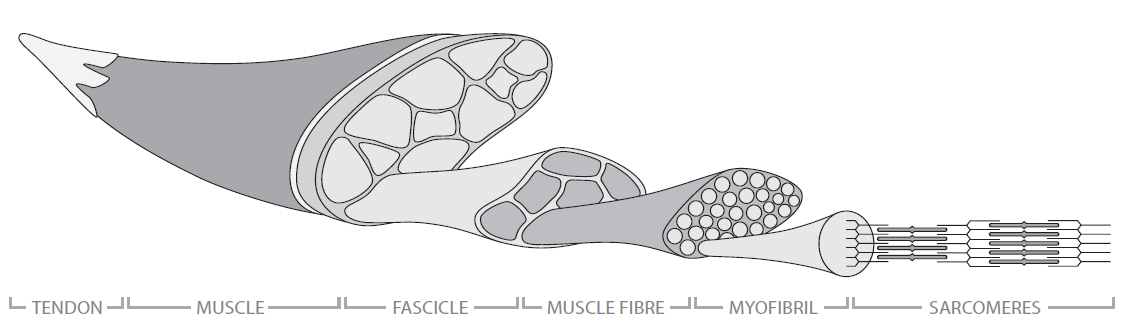
\includegraphics[scale=0.5]{muscleStructure.png}
	\caption{Major components of the muscle. Adapted from \citep{lee2010survey}.}
	\label{fig:muscleStructure}
\end{figure}
}

\subsection{Activation models}

\paragraph{}In order to simulate the muscle's contraction and generate force and movement, there are two main approaches: phenomenological and biophysical models \citep{tang20093d, rohrle2012physiologically}. Phenomenological models use mathematical and physics based constructs to describe the mechanical properties of biological tissue; in this case, skeletal muscles. One of the most used model is the Hill muscle model \citep{hill1970first}. This model is based on a series of experiments conducted on frog muscles, and captures the mechanical properties of the muscle. It has three major components: the series element (SE), the parallel element (PE), and the contractile element (CE). The series element (SE) represents mainly the elastic effects of tendon and intrinsic elasticity within the sarcomere. The parallel element (PE) represents the passive elasticity of the muscle resulting from the penetration of connective tissues into the muscle body. The contractile element (CE) accounts for generation of active force which is dependent on the muscle length, and the time-varying neural signal, a(t), originating from the central nervous system.

\paragraph{}On the contrary, biophysical models use physics to try to model biological systems. For muscle contraction, these models try to predict the muscle's response to a determinate stimulus. One commonly used biophysical model is the Huxley muscle contraction theory, that analyses the electrical activity of muscle fibers in order to generate movement. However, the Bidomain model \cite{rohrle2010simulating} is better suited at modelling the electric activity throughout a biological tissue. In the case of muscle contraction, based on a stimulus it calculates the muscle fiber's state before, during, and after a muscle contraction.

\subsection{State of the art}

\paragraph{}Since skeletal muscle are fundamental to maintain pose and to generate movement, there have been many studies that try to model the musculoskeletal system. For brevity, we will only mention the ones that have been relevant in the recent years.

\paragraph{}Lee and Terzopoulos \citep{lee2009comprehensive} developed a biomechanical model of the upper body. Their model is capable of modelling and controlling the muscles and bones, as well as simulating the physics-based deformations of the soft tissues. They incorporated 814 muscles, each of which is modeled as a piecewise uniaxial Hill-type force actuator. To simulate biomechanically-realistic flesh deformations, they developed a coupled finite element model with the appropriate constitutive behavior, in which are embedded the detailed 3D anatomical geometries of the hard and soft tissues. Finally, they created an associated physics-based animation controller that computes the muscle activation signals necessary to drive the elaborate musculoskeletal system in accordance with a sequence of target poses specified by an animator. A sample of their model can be seen in \fref{fig:muscleTorso}.

\afterpage{
\begin{figure}[t!]
	\centering
		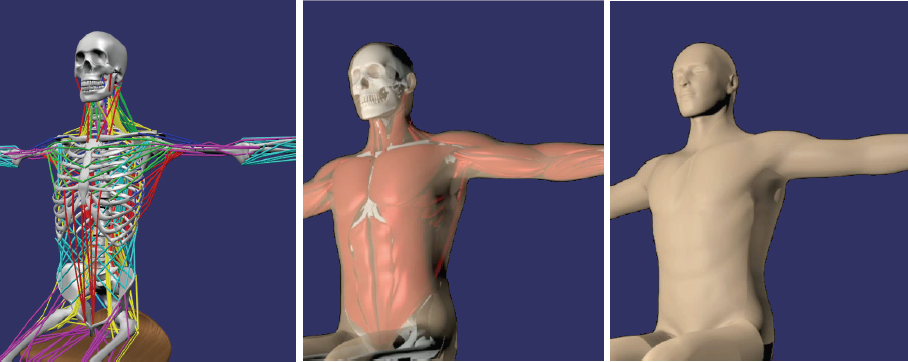
\includegraphics[scale=0.5]{muscleTorso.png}
	\caption{A skeleton moved by muscle modelled with a piecewise uniaxial Hill-type force actuator (left). The generated movement deforms the soft tissues (center), and the skin (right). Adapted from \citep{lee2009comprehensive}.}
	\label{fig:muscleTorso}
\end{figure}
}

\paragraph{}Unlike the work of Lee and Terzopoulos that use phenomenological models to generate force and movement, the work of Röhrle \citep{rohrle2010simulating, rohrle2012physiologically} uses the Bidomain model to describe the electrical activity and the subsequent contraction of the muscle fibers. The result is a physiologically based, multi-scale skeletal muscle finite element model that is capable of representing detailed, geometrical descriptions of skeletal muscle fibers and their grouping.

\paragraph{}Both previous works focus on a muscle model that has a physically based activation model, and use the Finite Element Method (FEM) to represent the muscle. The work of Fan et. al. \citep{fan2014active} focuses more on the visual accuracy rather than on the activation method. They introduce a framework for simulating the dynamics of musculoskeletal systems, with volumetric muscles in close contact and novel data-driven muscle activation model. Muscles are simulated using an Eulerian-on-Lagrangian discretization that handles volume preservation, large deformation, and close contact between adjacent tissues. Volume preservation is crucial for accurately capturing the dynamics of muscles and other biological tissues. Their model utilizes knowledge of the active shapes of muscles, which can be easily obtained from medical imaging data or designed to meet artistic needs. Their framework can be seen in \fref{fig:activeVolumetricMuscles}.

\afterpage{
\begin{figure}[t!]
	\centering
		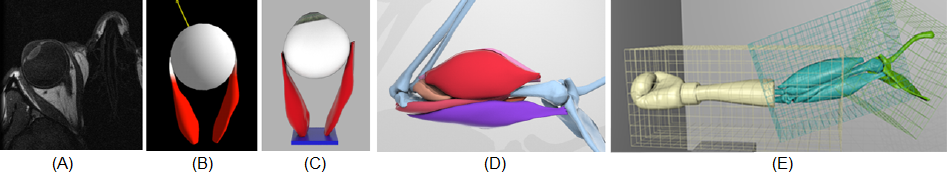
\includegraphics[keepaspectratio, scale=0.6]{activeVolumetricMuscles.png}
	\caption{The framework spans the entire pipeline for simulating volumetric musculoskeletal systems, starting from data on the active shapes of muscles to physically based simulation of muscles and soft tissues coupled to the skeletal system. The framework starts with muscle MRI data (A), then a reconstruction of the shape of the muscle is done in a 3D modelling software (B), and a simulation with the proposed method is generated (C). A set of six muscles of the arm are modelled (D), and those muscles are used in a dynamic simulation, with real bulging, tissue deformation, and contact with a simulated environment (E) \citep{fan2014active}.}
	\label{fig:activeVolumetricMuscles}
\end{figure}
}

\subsection{Problem statement}

\paragraph{}The musculoskeletal system consists of several biological structures, and is a crucial component for the analysis and simulation of human movement. However, it is inherently difficult to simulate this system, not just because of the complexity of the structures that conform it, but also because of all the relations between them that have to be taken into account.

\paragraph{}There are many challenges that have to be resolved in order to correctly simulate the musculoskeletal system. Some of them are as follows:

\begin{itemize}
	\item Most current simulations are simplifications of the overall system; either by simplifying the structures that the model uses, or the way they are controlled.  
	\item The way in which the tissues are simulated not always accounts for certain key properties, such as volume conservation, or bulging; or are simulated using techniques such as FEM, that are computationally expensive, and more so if such properties are to be considered.
	\item Most previous work does not model the muscle fibers, which are crucial for a correct muscle simulation.
	\item The mainly used activation methods are phenomenological. These are simplifications of the real behaviour of muscles, and have been proven to be wrong when comparing their output to real muscle output data. These models are more similar to simple mechanic systems than to biological systems. 
	\item The physical properties of the several components of the musculoskeletal system are normally not taken into account.
	\item Bones, ligaments, and tendons are either simplified or ignored for most simulations. 
\end{itemize}

\paragraph{}Currently, there does not exist a model of the musculoskeletal system that simulates the muscles considering their internal structure, the biological tissues that they are composed of, and their physical and biological properties, that is also activated using biophysical models that emulate how they respond to a signal from the nervous system. Additionally, most previous work focus on modelling a specific muscle, or a group of specific muscles, without providing a framework that can help model any muscle of the body.

\paragraph{}Furthermore, the computational cost to solve the different mathematical, and physical models, as well as the rendering of the various objects in the scene, can be high. However, not many studies rely on General Purpose computing on Graphics Processing Units (GPGPU), making their solutions not ideal for interactive or real time simulations.

\subsection{Proposed method}

\paragraph{}The first issue that needs to be solved is the simplification of the musculoskeletal system. We propose a model that encompasses several of the principal tissues and structures that are present in every muscle: the muscle fibers, connecting tissues, tendons, bone, and skin. Since the human body is comprised mostly of water, most of these tissues could be modelled using computational fluid dynamics (CFD) methods for fluid simulation. In this case, we propose the use of a modified Lattice Boltzmann Method (LBM) to model all the mentioned tissues. 

\paragraph{}Normally, the LBM models the flow of a fluid within a container. For this solution, the fluids are going to be the tissues of the body, each with their own material properties. We will use the lattice's speeds and material properties to simulate a very viscous, almost solid fluid, that modifies its container when needed (such as when an external force is present). This allows the tissue to have basic biological properties such as being deformable, incompressible, having volume preservation, and allowing the contact with other tissues.

\paragraph{}The proposed simulation of tissues requires the use of a very detailed human 3D model from which the containers can be obtained. We propose the use of BodyParts3D: 3D structure database for anatomical concepts \citep{mitsuhashi2009bodyparts3d} from the Database Center for Life Science \citep{DBCLS}. BodyParts3D is a dictionary-type database for anatomy in which anatomical concepts are represented by 3D structure data that specify corresponding segments of a 3D whole-body model for an adult human male. It encompasses morphological and geometrical knowledge in anatomy. BodyParts3D was constructed on the framework of a voxel human model for electromagnetic dosimetry, ‘TARO’, which was created from a whole-body set of 2 mm interval MRI images of a male volunteer.

\paragraph{}Once we have a model that is able to represent a biological tissue, we propose the use of a biophysical model in order to simulate the activation of the tissue. In the case of skeletal muscles, the Bidomain model has been used to model their electrical activity \citep{rohrle2012physiologically}. We will solve a Bidomain equation for each muscle fiber present in each muscle we simulate. However, since motor units innvervate several muscle fibers, a simplification where we only solve a bidomain model for each motor unit of the muscle could be considered.

\paragraph{}In order to test our proposed method, we will simulate two simple motion of one upper limb of a human body. We will simulate the extension and flexion of the arm around the elbow. We decided to simulate only said movements because they are produces by the activation of only a small number of muscles (biceps brachii, brachioradialis, brachialis, pronator teres, triceps brachii, and anconeus). However, our method could be applied to other muscles and could be used to produce a wide range of movements. 

\paragraph{}Finally, since we will have to solve several mathematical and physical models in order model the biological tissues and their activations, the use of GPGPU will be essential if we intend to produce an interactive simulation. We propose the use of the CUDA API to implement the LBM, and the Bidomain model. We will render all the elements of the simulation using shaders that also run on a Graphics Processing Unit (GPU). 














